\section{TECHNOLOGY REVIEW}

To achieve the goal of the work, necessary design and game elements have to be identified, to design an educational website that applies gamification principles to teach and drive recognition for open badges. 
While there is no exact example in the industry to follow for achieving this task, existing solutions of education and gamification applied in learning, digital badge systems will be reviewed, highlighting their core gamification features, similarities, and theories applied.

To develop the task, technology and software solutions will be reviewed for the website. 
Finally, the completion of the website's content is intended to reward the user with an open badge of their own. 
This means that an open badge creation pipeline solution will be reviewed, alongside metadata creation and its content to provide the website users with a token of verifiable completion that can be interoperably used across the Web.

\subsection{Review of Existing Similar Solutions}
Existing similar solutions will be reviewed to identify key features, gamified elements, and theoretical strategies relevant to designing them. For the purposes of the project, the only concern is with educational, gamification and open badge integrations. 
The analysis will focus on platforms utilizing features such as badges, progress tracking, and leaderboards and the approach to their design to identify key elements and features to be implemented. 
To provide depth, theoretical frameworks like \acrshort{sdt}, \acrshort{mda} Framework, flow theory and alternative approaches will be explored in their application to these platforms. 
This review will adopt a comparative analysis approach, organizing findings into four core criteria: platform name, gamification approach and features, theoretical foundations or strategies applied, and relevance to project goals. 
Aspects like Target Audience, Accessibility, strengths and weaknesses as well as many other potential outlines will be ignored due to being out-of-scope for the work.
Additionally, the selected products and services to-be-reviewed vary significantly in scope and application, so expanding the set of criteria to evaluate would lead to misrepresentation of certain criteria aspects.
By examining how these solutions address engagement and skill recognition, the review aims to conclude elements and strategies to inform the design of a gamified educational website about open badges.

Chart Criteria
\begin{itemize}
    \item \textbf{Platform Name and Type}:  Identify of the tool or platform and the type it represents..
    \item \textbf{Gamification and Features}:  Highlight applied game elements such as badges, leaderboards, progress tracking. Additionally track features, most notably open badge support and creation.
    \item \textbf{Theoretical Foundations or Strategies Applied}:  Examine the applied academic or practical design principles used to develop the features, to ensure evidence-based practices.
    \item \textbf{Relevance to Project Goals}: Explore relevance of application to the work, specifically in the field of recognition of achievement, recognition and integration of open badges. This ensures that actionable features and strategies are identified.
\end{itemize}


\begin{longtable}[c]{|p{3cm}|p{4.2cm}|p{4.2cm}|p{4.2cm}|}
\captionsetup{justification=raggedright, singlelinecheck=false}
\caption{Comparative Analysis of Existing Platforms} \\
\hline
\textbf{Platform Name, Type} & \textbf{Gamification and Features} & \textbf{Theoretical Foundations or Strategies Applied} & \textbf{Relevance to Project} \\
\hline
\endfirsthead
\hline
\textbf{Platform Name, Type} & \textbf{Gamification and Features} & \textbf{Theoretical Foundations or Strategies Applied} & \textbf{Relevance to Project} \\
\hline
\endhead
\hline
\endfoot
\hline
\endlastfoot

\textbf{Mozilla Open Badges, Open Badge System} & Open badge creation, sharing, verification. Supports rich metadata, dictates international standards for issuing badges for educational accreditations. & Open recognition and learner autonomy principles, which tie into \acrshort{sdt}. The focus is on creating a standardized system for recognition, with an emphasis on verifiability and interoperability. & Provides the technical infrastructure needed to issue, verify, and share digital badges as well as the necessary metadata standards dictated. \\
\hline
\textbf{Badgr (Canvas Badges), Open Badge System} & Badge issuance, progress tracking, \acrshort{lms} integration, and social sharing options. & Use of badges, achievements and progress tracking aligned with \acrshort{sdt} and flow theory. & Supports easy digital badge creation, tracking of and rewarding learning achievements on manageable tracks, highly relevant for hassle-free digital badge creation. \\
\hline
\textbf{Open Badge Factory, Open Badge System} & Badge creation, issuing, and sharing, with reporting and data analysis features. & Encourages engagement through earning, tracking, and rewarding achievements. & Directly aligns with the goal of creating and recognizing open badges, offering a clear example of implementing badge metadata. \\
\hline
\textbf{Duolingo, Language Learning App} & Badges, streaks, Experience points, leaderboards, interactive lessons, various types of time-based, performance-based, task and progress tracking. & \acrshort{sdt} application - user autonomy, setup for achieving competence, relatedness through social systems, MDA Framework for driving engagement. & Engages users with gamified visual elements - badges, trackers, a map of Units. Supports skill recognition through milestones, suggests that having multiple ways of tracking progress is likely important for the user to keep track of their progress. \\
\hline
\textbf{Khan Academy, Educational Platform} & Progress tracking, mastery points, badges, personalized dashboards. & Mastery-based learning, flow theory for balanced challenges and skill levels. & Emphasizes clear progress indicators and personalized learning paths for user motivation. \\
\hline
\textbf{Coursera, Online Learning Platform} & Courses with progress tracking, certificates, community engagement. & Constructivist(enable users to construct their own understanding of the topic) learning, social learning, \acrshort{sdt} application for intrinsic motivation. & Combines certification and achievement systems, ideal for integrating open badges. \\
\hline
\textbf{Classcraft, Gamified Learning Platform} & Role-playing game mechanics (Experience, level-ups), collaboration, quests, and rewards. Includes avatars, team-based challenges, and behaviour tracking. & \acrshort{sdt} - focuses on competence through skill mastery, autonomy via customizable avatars and quests, relatedness through team-based interactions. & Encourages engagement and motivation through collaboration and role-playing elements, ideal for promoting both individual and group-based achievements. \\ \hline 
\textbf{Habitica, Task and Habit Tracker} & Gamified to-do list with tasks, streaks, and rewards. Users earn experience points and rewards for completing real-life tasks and goals. & \acrshort{sdt} application - intrinsic motivation through task completion and goal setting, competence through measurable progress, autonomy in managing tasks. & Provides a fun, gamified way to encourage habit formation and task completion, suitable for user achievement tracking in everyday activities. \\ \hline 
\textbf{Kahoot!, Game-Based Learning Platform} & Interactive quizzes, surveys, polls, leaderboards, and real-time gameplay in classrooms or teams. & Active learning principles, \acrshort{sdt} through engagement and social interaction in competitive settings. & Facilitates real-time, competitive learning, ideal for assessing knowledge and encouraging participation in educational settings. \\ \hline
\end{longtable}
{\raggedright \small{Source:} compiled by the author\par}

Platforms Mozilla Open Badges, and Open Badge Factory, which provide standardized badge creation and management systems are both viable options for issuing the work-related open badges for the purposes of the project. 
Badgr seems like a great addition that could go on to improve the experience with simple extra digital badges to explain the difference between digital and open badges. 
These systems align with the goal of the project for open recognition of the final badge and digital achievement recognition.

Gamified applications like Duolingo, Classcraft, and Habitica are focused on incorporating interactive elements such as streaks, quests, progress trackers and experience points to motivate users. 
By applying \acrshort{sdt}, these platforms effectively enhance intrinsic motivation through autonomy and competence \cite{sdt}. 
Their emphasis on visual progress tracking and driving engagement highlights the importance of user-friendly interfaces for sustained participation. 
Duolingo’s gamified elements have been shown to increase user engagement and retention rates significantly.

Educational platforms Khan Academy and Coursera have developed personalized learning paths, mastery-based progress tracking, and social learning. 
These features are rooted in mastery learning, constructivist approaches, and active learning principles, which suggests the importance of personalized educational experiences that balance challenge and skill to maintain user engagement, per the flow theory \cite{flow}\cite{powerFeedback}. 
Unfortunately, personalizing learning paths and creating extensive social learning opportunities would not be viable for the project due to being considered out-of-scope for both aspects. 
Kahoot! and Classcraft emphasize collaborative and competitive learning, team-based interactions and real-time participation to encourage both individual and group achievements. 
While team-based interactions are also considered out-of-scope for the project, there is the opportunity to implement the playfulness of presenting educational content like they are done in both of these platforms to improve the user experience.

Overall, the findings suggest that combining the structured credentialing of open badge systems with the engaging, user-centric design of gamified platforms can create an intuitive framework for motivated learning. 
These strategies and practical insights will serve as the foundation for designing an educational platform that integrates gamification and achievement recognition to drive both user engagement and educational outcomes.

\subsection{Technology Review}

\begin{enumerate}
  \addtolength{\itemsep}{-0.5\baselineskip} 
  \item {Gamification and Motivation.} \acrshort{sdt}, flow theory and \acrshort{mda} will be applied for the design of the gamified website, in the forms of progress tracking, leaderboard (completion time) and rewards (the digital and open badges)\cite{sdt}\cite{flow}.
  \item {Open Badges and Digital Credentialing.} Digital badges will be created and issued using international metadata standards outlined by the Mozilla Open Badges. 
  A pursuit to create them through automatic means will then be made, whether with one of the available tools (Mozilla Open Badges, Badgr, Open Badge Factory).
  \item {User Experience and Interface Design.} A user interface will be implemented for user flow and driving user engagement. 
  The standard goal for the user interface will be a successful application of \acrshort{fbm} \cite{fogg}, which is focused on three key factors: motivation, ability and triggers. 
  Simplicity is crucial to \acrshort{fbm}  to reduce friction and drive user engagement. 
  To further illustrate this, Figure \ref{fig:foggChart} \footnote{https://behaviormodel.org/} shows that specifically, a balance of the three barriers is necessary. 
  So by making the platform more approachable and visually appealing, minimising barriers and using user-centric design, it is possible to improve learning follow-through.
  \item {Responsive Web Design.} The website will be designed mobile-first with relevant principles, as that is where most people are likely to experience the content according to Prakash (2020) \cite{mobileDesign}. 
\end{enumerate}

\begin{figure}[htbp]
 \centering
 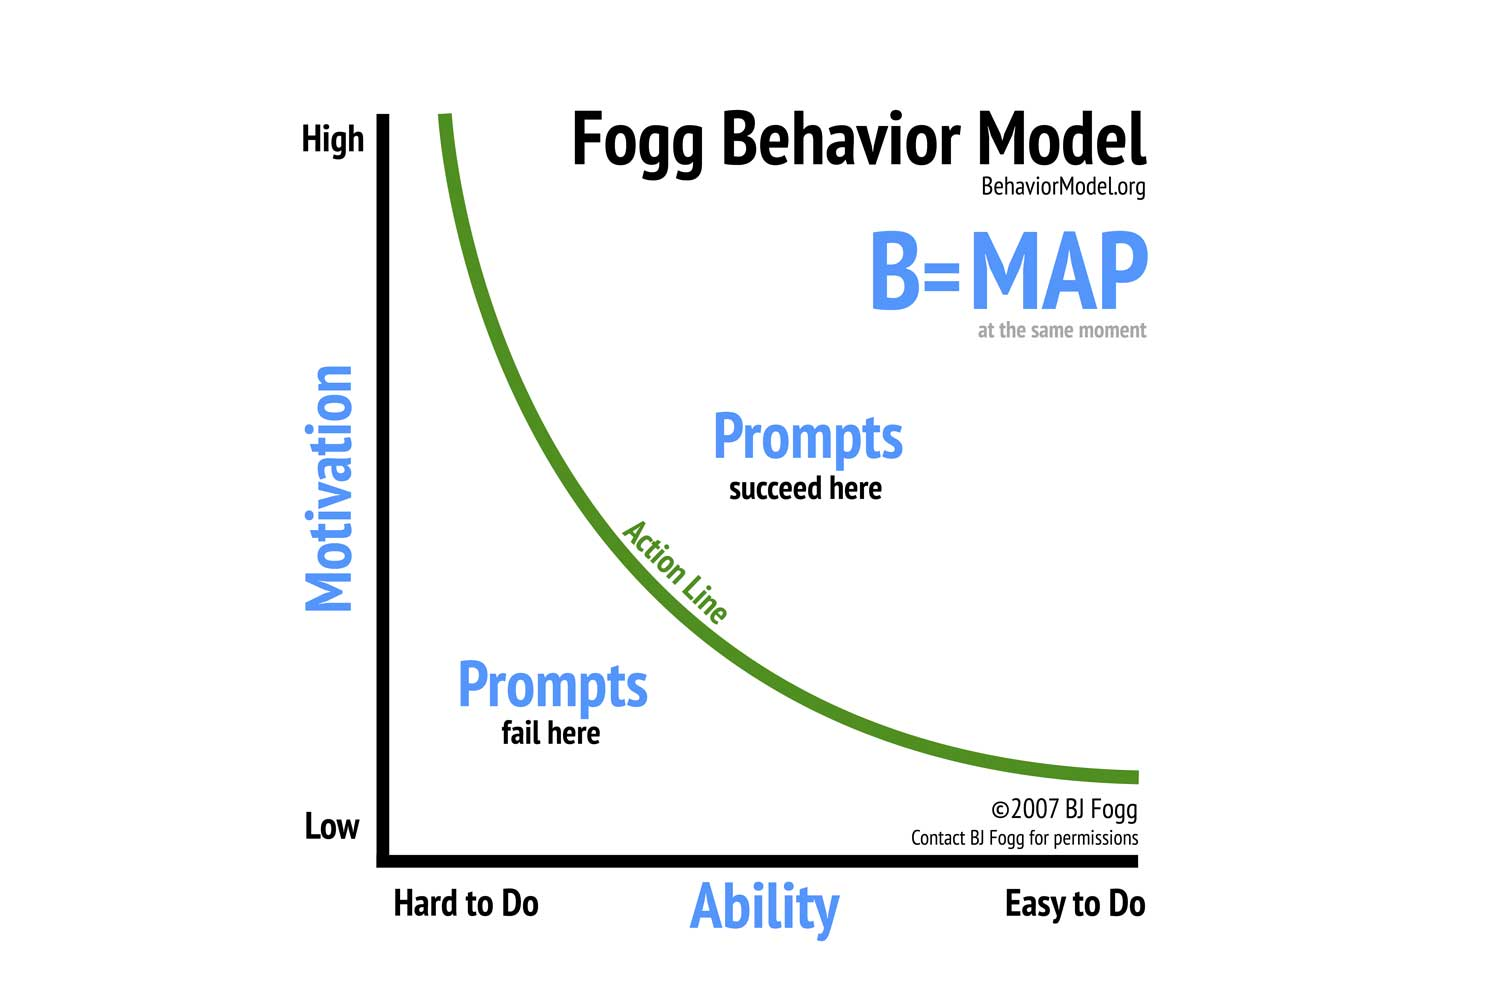
\includegraphics[width=14cm]{Media/Fogg-Behavior-Model.jpg}
 \caption{Fogg's Behavior Model}
 \label{fig:foggChart}
 {\raggedright \small{Source:} behaviormodel.org, 2009\par}
\end{figure}

\subsection{Website Characteristics Review}

\begin{enumerate}
    \item \textbf{User Engagement and Motivation:} 
    \begin{itemize}
        \item \textbf{Gamified Elements.}
        \begin{itemize}
            \item Streaks. The website is planned to be completed relatively quickly, so to maintain better user engagement, streaks will be used that will trigger after every completed task or minigame, that will play a stair-climbing animation. The said animation will consistently increase the climbing speed up to completion.
            \item Leaderboards. In the event of tracking user completion speeds and success rates, a leaderboard using their created usernames will be made available after completion or from the landing page menu.
            \item Progress bars and trackers. Progress trackers will be visible within tasks and between them so that users can clearly understand their current state and progress.
            \item Rewards. Digital and Open badges will be rewarded along the way, so the user feels rewarded for their efforts.
        \end{itemize}
        \item \textbf{User-Centric Design.}
        \begin{itemize}
            \item Simple layout with minimal visual elements, that streamlines the experience.
            \item Strict on-rails experience that should lead to higher completion rates of the lessons.
        \end{itemize}
        \item \textbf{Immediate Feedback.}
        \begin{itemize}
            \item Quick-paced tasks with real-time responses to user actions.
            \item Responsive tasks with direct and specific feedback regarding wrong options.
            \begin{itemize}
                \item An example of this could be a question with multiple choice answers, where there is a correct, wrong and witty answer, that would each reward the user with a respective digital badge. This would also allow for displaying the multifaceted prowess of the website for the user.
            \end{itemize}
        \end{itemize}
    \end{itemize}
    % -----------------------------------------------------------
    \item \textbf{Educational Effectiveness:}
    \begin{itemize}
        \item \textbf{Interactive Learning.}
        \begin{itemize}
            \item Quizzes. Each module will feature interactive quizzes designed to test knowledge and introduce new information.
            \item Minigames. There are currently 2 planned minigames that would introduce a change of pace, drive further engagement, and be tied to the topic in a way so that the user can be seamlessly further educated.
        \end{itemize}
        \item \textbf{Scenario-Based Learning.} Lessons will be related to real-world scenarios that require users to make choices or solve problems, keeping the learning process dynamic and engaging.
        \item \textbf{Branching Path.} While the planned scope is estimated to be relatively small, an introduction of a branching path that allows the user to take on different tasks could lead to further engagement. 
        This would additionally create the feeling of a proper \acrshort{lms} for the user. 
        The branches would ultimately either converge at the same point or provide the option to complete both branches.
        \item \textbf{Onboarding and Tooltips.}
        \begin{itemize}
            \item Contextual help popups. The website will include tooltips and minimal onboarding to guide the user, further reducing learning friction.
        \end{itemize}
    \end{itemize}
    % -----------------------------------------------------------
    \item \textbf{Design Choices:}
    \begin{itemize}
        \item \textbf{Language.} The website will be written entirely in Lithuanian, with considerations for localization in English.
        \item \textbf{Animations.}
        \begin{itemize}
            \item Welcome animation. Upon landing on the website, users will see an animated introduction explaining the value of badges and their role in the learning process. 
            This will immediately engage users and explain the educational context.
            \item Animation of badges combining. To be played to explain a certain aspect of open badges.
            \item Final reward animation. Receiving the necessary amount of badges and completing the required steps will lead to an open badge reward that will be awarded with an animation.
            \item Animations will be achieved both via direct code and creation through alternative applications.
        \end{itemize}
        \item \textbf{Badge Collection Display.}
        \begin{itemize}
            \item Grid display. Earned badges will be displayed in an interactive grid, which users can click on to view details and metadata. 
            This will give users further understanding of digital and open badges.
        \end{itemize}
    \end{itemize}
    % -----------------------------------------------------------
    \item \textbf{Design Elements:}
    \begin{itemize}
        \item \textbf{Colors.} A clean and vibrant color palette will be used to enhance the visual appeal. 
            \begin{itemize}
            \item Exact color palettes are to be explored later. 
            \item Blue and white are likely guaranteed colors due to the association to the university's open badge system color scheme. 
            \item Red is guaranteed for error display.
            \end{itemize}
        \item \textbf{Art.} The website is planned to utilize primarily vector art.
        \item \textbf{Typography.} 
            \begin{itemize}
            \item Simple, sans-serif fonts will be used for readability. 
            \item The main body text will be light. 
            \item Headings will be bold to create a visual hierarchy.
            \end{itemize}
        \item \textbf{Visual Elements.} Icons will be used throughout the platform to represent different tasks, badges, and achievements.
    \end{itemize}
\end{enumerate}
%

\subsection{Software Solution Review}
%
As of writing this, the software solutions are subject to change, but are based on previous work and current knowledge and skills. 
The list of software implies that the software may be applied either in combination or by selection, and alternative options may be considered during development.\\
%

\begin{itemize}
    
    \item \textbf{Web Technologies:} 
    \begin{itemize}
        \item HTML5, CSS3, and JavaScript: Core technologies for building a responsive and engaging frontend, ensuring cross-browser compatibility and user interaction independent of platform of choice.
        \item Node.js with Express: Efficient and scalable backend development API for handling data, user authentication and game logic.
    \end{itemize}
    
    \item \textbf{API Integrations:}
    \begin{itemize}
        \item Open Badge Standard APIs: Facilitates seamless badge issuance, verification, and sharing.
        \item Open Badge Factory API: For badge creation, maintenance and delivery via email.
    \end{itemize}
    
    \item \textbf{Example Software Solution:}
    \begin{itemize}
        \item React.js: A robust framework for building dynamic, modular, and responsive user interfaces.
        \item Node.js/Express: Manages server-side logic, API endpoints, and business processes.
        \item Git CI/CD Tools: Automates testing and deployment processes for consistent and reliable updates.
    \end{itemize}
    
    \item \textbf{Other Tools and Considerations:}
    \begin{itemize}
        \item Version Control: Git for collaborative development and version tracking.
        \item Testing Frameworks: Jest or Mocha for unit testing frontend and backend components.
        \item Accessibility Testing will be considered: Lighthouse or Axe tools to ensure compliance with accessibility standards (e.g., WCAG).
    \end{itemize}
\end{itemize}